
\documentclass{article}
\usepackage{amsmath, amssymb, tikz, graphicx}
\usepackage[margin=2.5cm]{geometry}
\usepackage{booktabs}

\title{Kategorientheoretisches Buchhaltungsmodell mit Makroinvarianz}
\author{Generated by ChatGPT for Viktor}
\date{\today}

\begin{document}
\maketitle

\section*{Theoretischer Teil}

Wir modellieren Agenten mit doppelter Buchführung als Objekte in einer Kategorie \( \mathcal{A} \).\\newline
Die Transaktionen zwischen Agenten werden als Morphismen in dieser Kategorie beschrieben. Die Kategorie ist wie folgt aufgebaut:

\begin{itemize}
  \item \textbf{Objekte}: MicroLedger \( L_i = (A_i, L_i) \) mit Aktiv- und Passivkonten
  \item \textbf{Morphismen}: MicroBookings \( b: A \to B \)
  \item \textbf{Pattern}: Diagramme aus diesen Morphismen
  \item \textbf{Bindings}: konkrete Werte wie Betrag und Kontenbindung
  \item \textbf{Colimit}: aggregierter Zustand, in dem alle Morphismen verklebt sind und die Makroinvarianz prüfen
  \item \textbf{Natürliche Transformation}: \( \mu: F \Rightarrow G \), mit \( \mu_i = \text{microledger\_balance} \)
\end{itemize}

\section*{Praxisbeispiel: Zwei Buchungen}

Wir betrachten zwei Transaktionen zwischen Händler und Bank.

\subsection*{1. Waren gegen Warenschein}

\begin{itemize}
  \item Agent A (Händler) liefert Ware (Aktiva)
  \item Agent B (Kunde) erhält Warenschein (Verbindlichkeit)
\end{itemize}

\[
\text{Buchung:} \quad A: \text{debit } 100 \longrightarrow B: \text{credit } 100
\]

\begin{center}
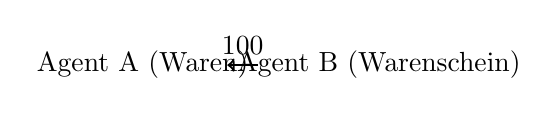
\begin{tikzpicture}[->, node distance=3cm]
  \node (A) {Agent A (Waren)};
  \node (B) [right of=A] {Agent B (Warenschein)};
  \draw[->, thick] (A) -- node[above]{100} (B);
\end{tikzpicture}
\end{center}

\[
\mu_A = +100, \quad \mu_B = -100, \quad \sum \mu_i = 0
\]

\subsection*{2. Geld gegen Kredit}

\begin{itemize}
  \item Agent A (Bank) vergibt Kredit in Geld
  \item Agent B (Kunde) erhält Geld, schuldet Kredit
\end{itemize}

\[
\text{Buchung:} \quad A: \text{debit } 50 \longrightarrow B: \text{credit } 50
\]

\begin{center}
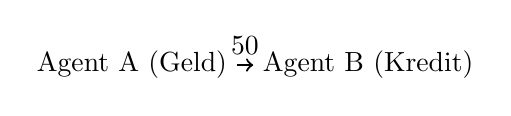
\begin{tikzpicture}[->, node distance=3cm]
  \node (A2) {Agent A (Geld)};
  \node (B2) [right of=A2] {Agent B (Kredit)};
  \draw[->, thick] (A2) -- node[above]{50} (B2);
\end{tikzpicture}
\end{center}

\[
\mu_A = +50, \quad \mu_B = -50, \quad \sum \mu_i = 0
\]

\section*{Rollenspezifikation}

\begin{description}
  \item[Buchhalter:] Jede Buchung ist ein Soll-/Haben-Vorgang in der doppelten Buchführung.
  \item[Programmierer:] Die Buchung ist eine Mutationsfunktion über Zustandsobjekte.
  \item[Kategorientheoretiker:] Morphismusdiagramme, Funktoren und Colimits prüfen strukturelle Konsistenz.
  \item[Investor:] Finanzflüsse sind sichtbar und quantitativ nachvollziehbar.
\end{description}

\end{document}
